\chapter{Background}

In this chapter, we introduce some of the techniques we use in the following
chapters. 
%
In particular, we describe a form of supervised learning, classification, and of
unsupervised learning, clustering.
%
We also describe the use of {\em word embeddings}, in particular, the modern use
of neural network-based word embeddings, such as {\em word2vec} and {\em
fastText}.


\section{Supervised learning: Classification}

The basic premise of learning from data is the use of a set of observations to
uncover an underlying process~\cite{Abu-Mostafa:2012:LD:2207825}. 
%
More formally, a way to see this is finding a function that optimizes certain
score, based on the available data. 
%
This function can be seen as an approximation of the real, unknown function
that describes the process that generates the data.

%%

When the {\em training data} (the available data) contains explicit examples of
what the correct output should be, then we are within the supervised learning
setting.
%
In this setting, classification is the process to assign a certain {\em label}
to an observation, or data point, in order to categorize it into a certain class
or category.
%
A {\em classifier} is a particular instance of the process, which can be {\em
trained} from a set of previously labeled observations in order to set its
appropiate parameters.
%
The output of a classifier applied to an observation is the label corresponding
to that observation (Figure~\ref{background:fig:clf-ex}).
%
Formally, a classifier is a function $h: \mathcal{D} \rightarrow \{0, 1, \ldots,
n\}$ which tries to approximate to the {\em real} function $f$.
%
A {\em binary classifier} is a function restricted to only two labels, $h:
\mathcal{D} \rightarrow \{0, 1\}$.
%
The training process of a classifier corresponds to find a function $h$ from a
{\em hypothesis set} $\mathcal{H}$ which contains all possible functions based
on the selected {\em model}.
%
For example, $\mathcal{H}$ would be all quadratic functions $h(x) = ax^2 + bx +
c$, and the goal is to find the correct set of parameters $(a, b, c)$ that make
$h$ fit the training data.
%
An error measure that is commonly used is the squared error: $e(h) =
(h(\vect{x}) - f(\vect{x}))^2$.
%
As we do not know $f$, the error measure is only an approximation of the real
error, which is called {\em in-sample error}, while the real error is called
{\em out-of-sample error}.
% 
There are models that estimate bounds for which the in-sample error can
approximate the out-of-sample error.
%
In the binary setting, the Vapnik–Chervonenkis (VC) dimension~\cite{Vapnik2015}
is an estimation on how well a function $h$ from a hypothesis set can fit a set
of data points, based on the characteristics of $\mathcal{H}$ and the number of
data points.

%
\begin{figure}
    \centering
    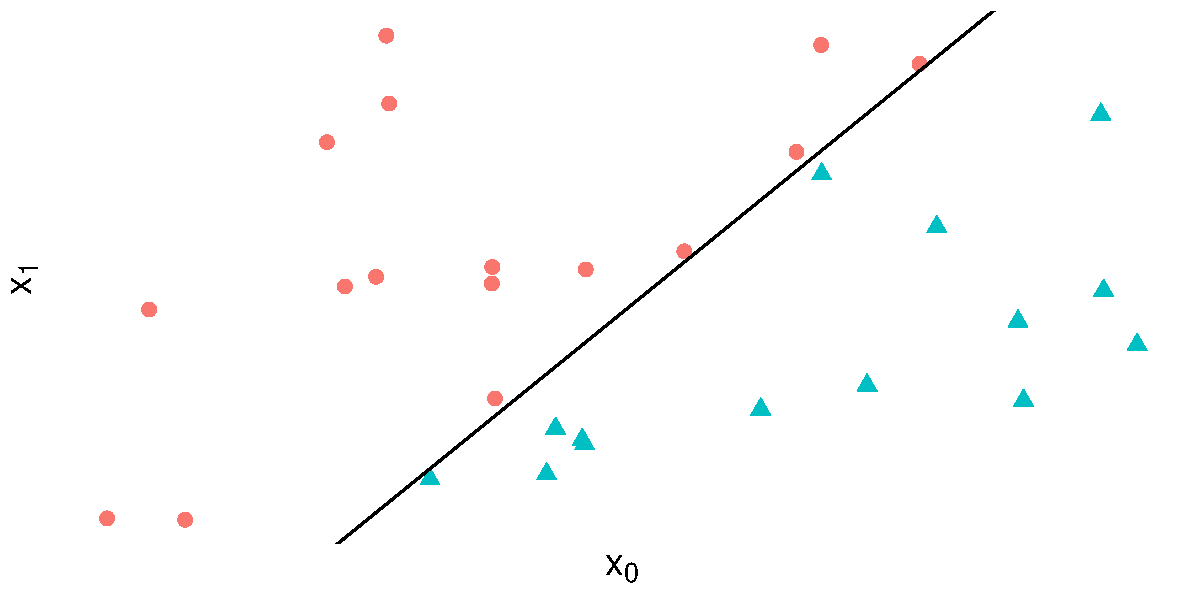
\includegraphics[width=.8\textwidth]{figures/background/classification-example}
    \caption{Example of classification as a decision boundary.}
    \label{background:fig:clf-ex}
\end{figure}%


\paragraph{Linear model.} The linear model is the family of functions (or
hypothesis set) defined as $h(\vect{x}) = \vect{w}^\customT\vect{x}$, where
$\vect{w} \in \mathbb{R}^\textit{d}, \textit{d} > 0$ is a vector of weights, and
$\vect{x}\in \mathbb{R}^\textit{d}$ is an observation. 
%
The {\em perceptron} is defined as $h(\vect{x}) =
\text{sign}(\vect{w}^\customT\vect{x})$, which is the foundation of several
linear models and neural network models.

%%

The perceptron uses a hard threshold on the signal $s =
\vect{w}^\customT\vect{x}$ by taking the sign of $s$ in order to perform linear
classification.
%
{\em Linear regression} outputs a real value by using the signal $s$ as the
output, $h(\vect{x}) = \vect{w}^\customT\vect{x}$.
%
{\em Logistic regression} restricts the output to the range $[0, 1]$, making
it interpretable as a probability: $h(\vect{x}) =
\theta(\vect{w}^\customT\vect{x})$, where $\theta$ is the so-called logistic
function, $\theta(s) = \frac{e^s}{1 + e^s}$.
%
There are several other linear models, which we will not mention in this brief
summary, but some of them can be studied
online\footnote{\url{https://scikit-learn.org/stable/modules/linear_model.html}
(Accessed: April 8, 2019)}.

%%

There are different learning algorithms in each case. 
%
For the perceptron, there is the {\em Perceptron Learning Algorithm} and the
{\em Pocket Algorithm}~\cite{Abu-Mostafa:2012:LD:2207825}. 
%
For the linear regression, a exact analytic expression can be derived by
minimizing the in-sample error, $E_{\text{in}}(h) = \frac{1}{N} \sum_{n=1}^{N}
(h(\vect{x}_n) - y_n)^2$, where $y_n = f(\vect{x}_n)$ is the label of the $n$-th
observation.
%
For logistic regression, the {\em gradient descent algorithm} provides a way to
find a local optimum for the in-sample error $E_{\text{in}}(h)$, which is
defined as the cross-entropy measure between $h(\vect{x})$ and $y$. 

%%

Gradient descent is a general technique for minimizing a twice-differentiable
function. 
%
It is performed by computing the gradient of the in-sample error $\nabla
E_{\text{in}}(h)$, and ``moving'' the weight vector according to the direction
of the gradient, $\vect{w}_{t+1} = \vect{w}_t - \eta\nabla E_{\text{in}}(h)$.
%
There are several strategies to stop the iteration $t$, such as doing it until
the change is small, a fixed number of times, or when the error is small enough.
%
The magnitude of the movement is given by the parameter $\eta$, or {\em learning
rate} which is usually a fixed value.


\paragraph{Neural network models.} 


\section{Unsupervised learning: Clustering}

Clustering algorithms group a set of documents into subsets or {\em
clusters}~\cite{manning2010introduction}.
%
The goal of the algorithms is to produce clusters that are internally coherent,
while very different from each other.
%
Clustering is the most common form of unsupervised learning, when we do not have
the exact labels corresponding to each observation. 
%
In this case, it is the features in the data which will correlate to the labels.
%
Our goal is to replicate the distinction that a human observer would impose on
the data.


\paragraph{K-Means.} 
%

%


\paragraph{Hierarchical clustering.}

\paragraph{Online clustering.}

\section{Neural Network-based Word Embeddings}